\section{Music Theory}

\blockquote{``Right from the start, it is important to learn how to write down music clearly. As a musician, unclear manuscript can waste valuable rehearsal time and might lead to performance mistakes. In an exam, badly written work may be misunderstood and could lose you vital marks.'' \parencite{taylor1989ab}}

For early grades of music theory, the criteria by which students need to adhere in order to maximize their marks and musical potential is covered in quite specific detail. This makes sense as the majority of students taking the exam are likely to be young and since they are also unlikely to have encountered much written music before, this is the most crucial time for teaching them good habits.

The following is a guide to the manuscript entities that a student aiming to take their grade 1 - 3 theory exams would most likely have to know about and/or write down, along with the relevant criteria for what constitutes acceptable and unacceptable manuscript, most of the examples below are taken from or based on the official documentation in \parencite{taylor2008music}

\todo[inline, color=red]{CURRENTLY SPLITTING THIS INTO TWO SECTIONS, first an overview of JUST music theory, THEN a section on things which students regularly get wrong, backed up by examples from the books and the data gathered from teachers like in \cref{fig:teacher-example-quaver-wrong-side}}

\subsection{Notes on the stave}

\subsubsection{Staves and Staff Lines}
\todo[inline,color=red]{Background - Music Stave}
\label{sec:music-theory-stave}

\subsubsection{Semibreve}

The semibreve is the easiest note to draw and is simply an oval outline, however, the rules which govern it's placement are quite specific as outlined in Figures \cref{fig:SemibreveOnLine} \& \cref{fig:SemibreveOnSpace}

\begin{figure}[h!]
  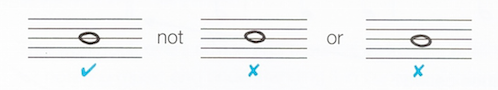
\includegraphics[width=\linewidth]{gfx/basic/semibreve-on-line.png}
  \centering
  \caption{If it is drawn on the line, the line must go exactly through the middle of the semibreve}
  \label{fig:SemibreveOnLine}
\end{figure}

\begin{figure}[h!]
  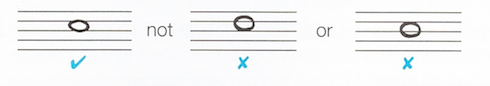
\includegraphics[width=\linewidth]{gfx/basic/semibreve-on-space.png}
  \centering
  \caption{If it is drawn in the space, it should also only cover half the space on either side}
  \label{fig:SemibreveOnSpace}
\end{figure}

\subsubsection{Ledger Lines}

Notes can be drawn higher or lower than the five stave lines by drawing another line or lines above or below the stave.

\begin{figure}[h!]
  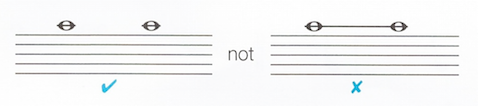
\includegraphics[width=\linewidth]{gfx/basic/ledger-boundaries.png}
  \centering
  \caption{Each note must have it's own line restricted to the boundaries of the note}
  \label{fig:LedgerBoundaries}
\end{figure}


\begin{figure}[h!]
  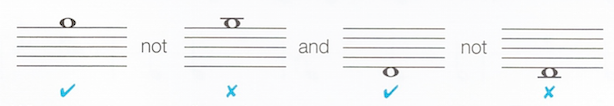
\includegraphics[width=\linewidth]{gfx/basic/ledger-above.png}
  \centering
  \caption{Lines should not be drawn over notes just above the stave, or below a note just under the stave}
  \label{fig:LedgerAbove}
\end{figure}


\begin{figure}[h!]
  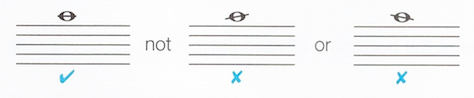
\includegraphics[width=\linewidth]{gfx/basic/ledger-slope.png}
  \centering
  \caption{The lines you draw through notes should not slope up or down, but should be exactly horizontal}
  \label{fig:LedgerSlope}
\end{figure}

\subsection{Stems}

The stem of a note should go up on the right and down on the left. Which version to use depends on which line the head of the note is placed upon.

The stems of the notes on the top two lines should go down
The stems of the notes on the bottom two lines should go up
The stems of the notes on the middle line can go either up \emph{or} down.

\begin{figure}[h!]
  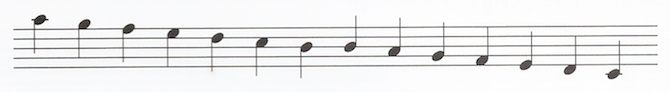
\includegraphics[width=\linewidth]{gfx/basic/stems-chromatic.png}
  \centering
  \caption{Examples of note stem direction}
  \label{fig:StemsChromatic}
\end{figure}

How the stems are drawn is quite important as they must not be too long or too short and should be vertically straight.

\begin{figure}[h!]
  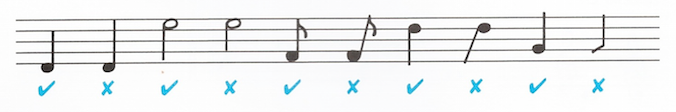
\includegraphics[width=\linewidth]{gfx/basic/stems-good-bad.png}
  \centering
  \caption{Examples of good and badly drawn note stems}
  \label{fig:StemsGoodBad}
\end{figure}

Quavers and eighth notes have small tails on them, typically in printed music they're curved but for handwritten notation straight lines are perfectly acceptable.

\begin{figure}[h!]
  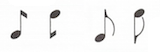
\includegraphics[width=0.4\linewidth]{gfx/basic/stems-curved.png}
  \centering
  \caption{Examples of straight and curved note stems}
  \label{fig:StemsStraightCurved}
\end{figure}

\subsection{Clefs}

\subsubsection{Treble Cleff}

The treble clef is one of the more difficult symbols to master, but has a fairly straightforward technique. You start with a loop around the \emph{G} line (second from the bottom) and then follow through with the loops.

\begin{figure}[h!]
  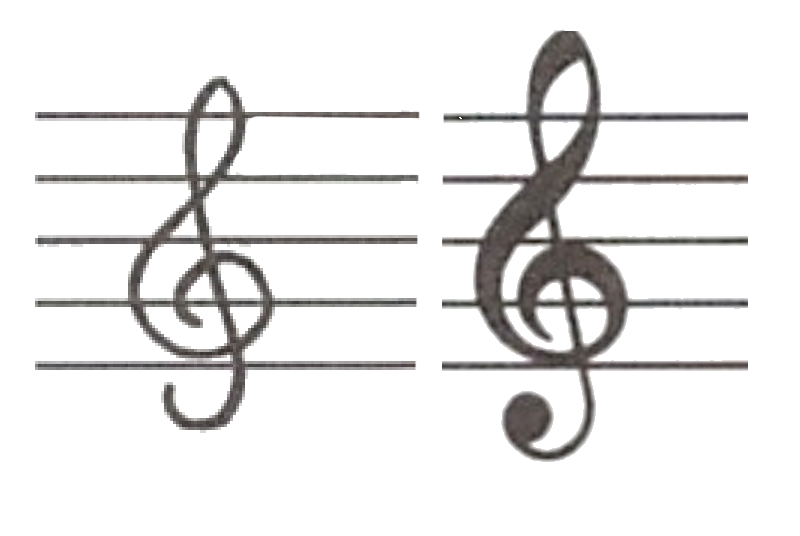
\includegraphics[width=0.3\linewidth]{gfx/basic/treble-clef.png}
  \centering
  \label{fig:TrebleClef}
\end{figure}

\subsubsection{Bass Clef}

The bass clef has two different variations, both with two dots to the right, either side of the \emph{F} line (second from the top) around which the core of the clef is centered. The left variation is by far the most common.

\begin{figure}[h!]
  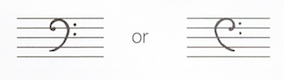
\includegraphics[width=0.5\linewidth]{gfx/basic/bass-clef.png}
  \centering
  \caption{Two versions of the Bass Clef}
  \label{fig:BassClef}
\end{figure}

\subsection{Beaming}

Notes with tails are often joined together, known as \emph{beaming}. For example, you can beam the following notes together:

\begin{figure}[h!]
  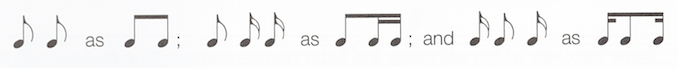
\includegraphics[width=\linewidth]{gfx/basic/beaming.png}
  \centering
  \caption{Notes and their beamed equivalents}
  \label{fig:NotesBeamedEquiv}
\end{figure}


\subsection{Rests}

\begin{enumerate}
\item The semibreve rest hangs below a line (usually the fourth) and is depicted by a rectangle which fills half the line space.
\item The minim rest is depicted similarly, but above the line (usually the third)
\end{enumerate}

\begin{figure}[h!]
  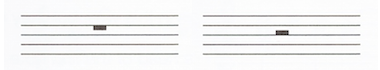
\includegraphics[width=0.7\linewidth]{gfx/basic/semibreve-minim-rest.png}
  \centering
  \caption{Examples of the semibreve rest (left) and minim rest (right)}
  \label{fig:RestMinimSemibreve}
\end{figure}

You can draw a crochet one of two ways and although the first is harder to draw, it is the most commonly used, so is the preferred version when learning to write music. This, and examples of a quaver and semiquaver rest can be seen in Figure \cref{fig:RestCrochetQS}

\begin{figure}[h!]
  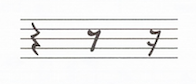
\includegraphics[width=0.5\linewidth]{gfx/basic/rests.png}
  \centering
  \caption{Examples of crochet, quaver and semiquaver rests}
  \label{fig:RestCrochetQS}
\end{figure}

\subsection {Ties}

A tie joins notes which sound the same and turns them into one sound. For example:

\begin{figure}[h!]
  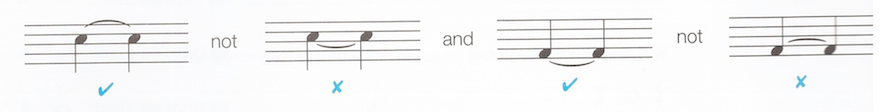
\includegraphics[width=\linewidth]{gfx/basic/ties.png}
  \centering
  \caption{Example of tied notes}
  \label{fig:TiedNotes}
\end{figure}

You can join any number of notes in this way, but they must be the same notes and they must be next to each other, the tie goes from the head of the first note to the head of the next.

\subsection{Dotted Notes}

Dotted notes are very simple to draw and their purpose is even simpler. They make any dotted note equal to 1.5 $\times$ the length of the same note without the dot.

\begin{figure}[h!]
  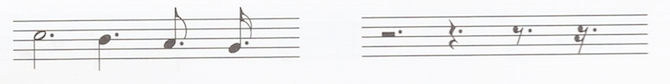
\includegraphics[width=\linewidth]{gfx/basic/dotted-notes.png}
  \centering
  \caption{Dotted Notes}
  \label{fig:DottedNotes}
\end{figure}

\subsection{Accidentals}

When placed on staff lines or spaces, accidentals modify the note which they precede. They must lie evenly across a line or a space because as with previous notation, bad placement leads to ambiguity an lost marks

\begin{enumerate}
\item Sharps modify a note by adding a semitone to it's original value
\item Flats modify a note by subtracting a semitone to it's original value
\item Naturals modify a note by removing the influence of any previous sharps or flats.
\end{enumerate}

\begin{figure}[h!]
  \centering
  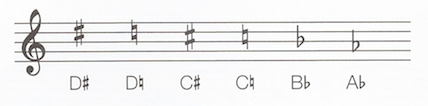
\includegraphics[width=\linewidth]{gfx/basic/accidentals.png}
  \caption{Examples of accidentals}
  \label{fig:Accidentals}
\end{figure}


\section{Common Manuscript Mistakes}
\todo[inline,color=red]{Most of the screenshots from before will go here, and the example for the music theory overview will be replaced with actual manuscript notation examples or printed examples}

\todo[inline,color=red]{Talk more about the teacher sheets like \cref{fig:teacher-sheet} and refer to them in scoring section}

\begin{figure}[H]
  \rot{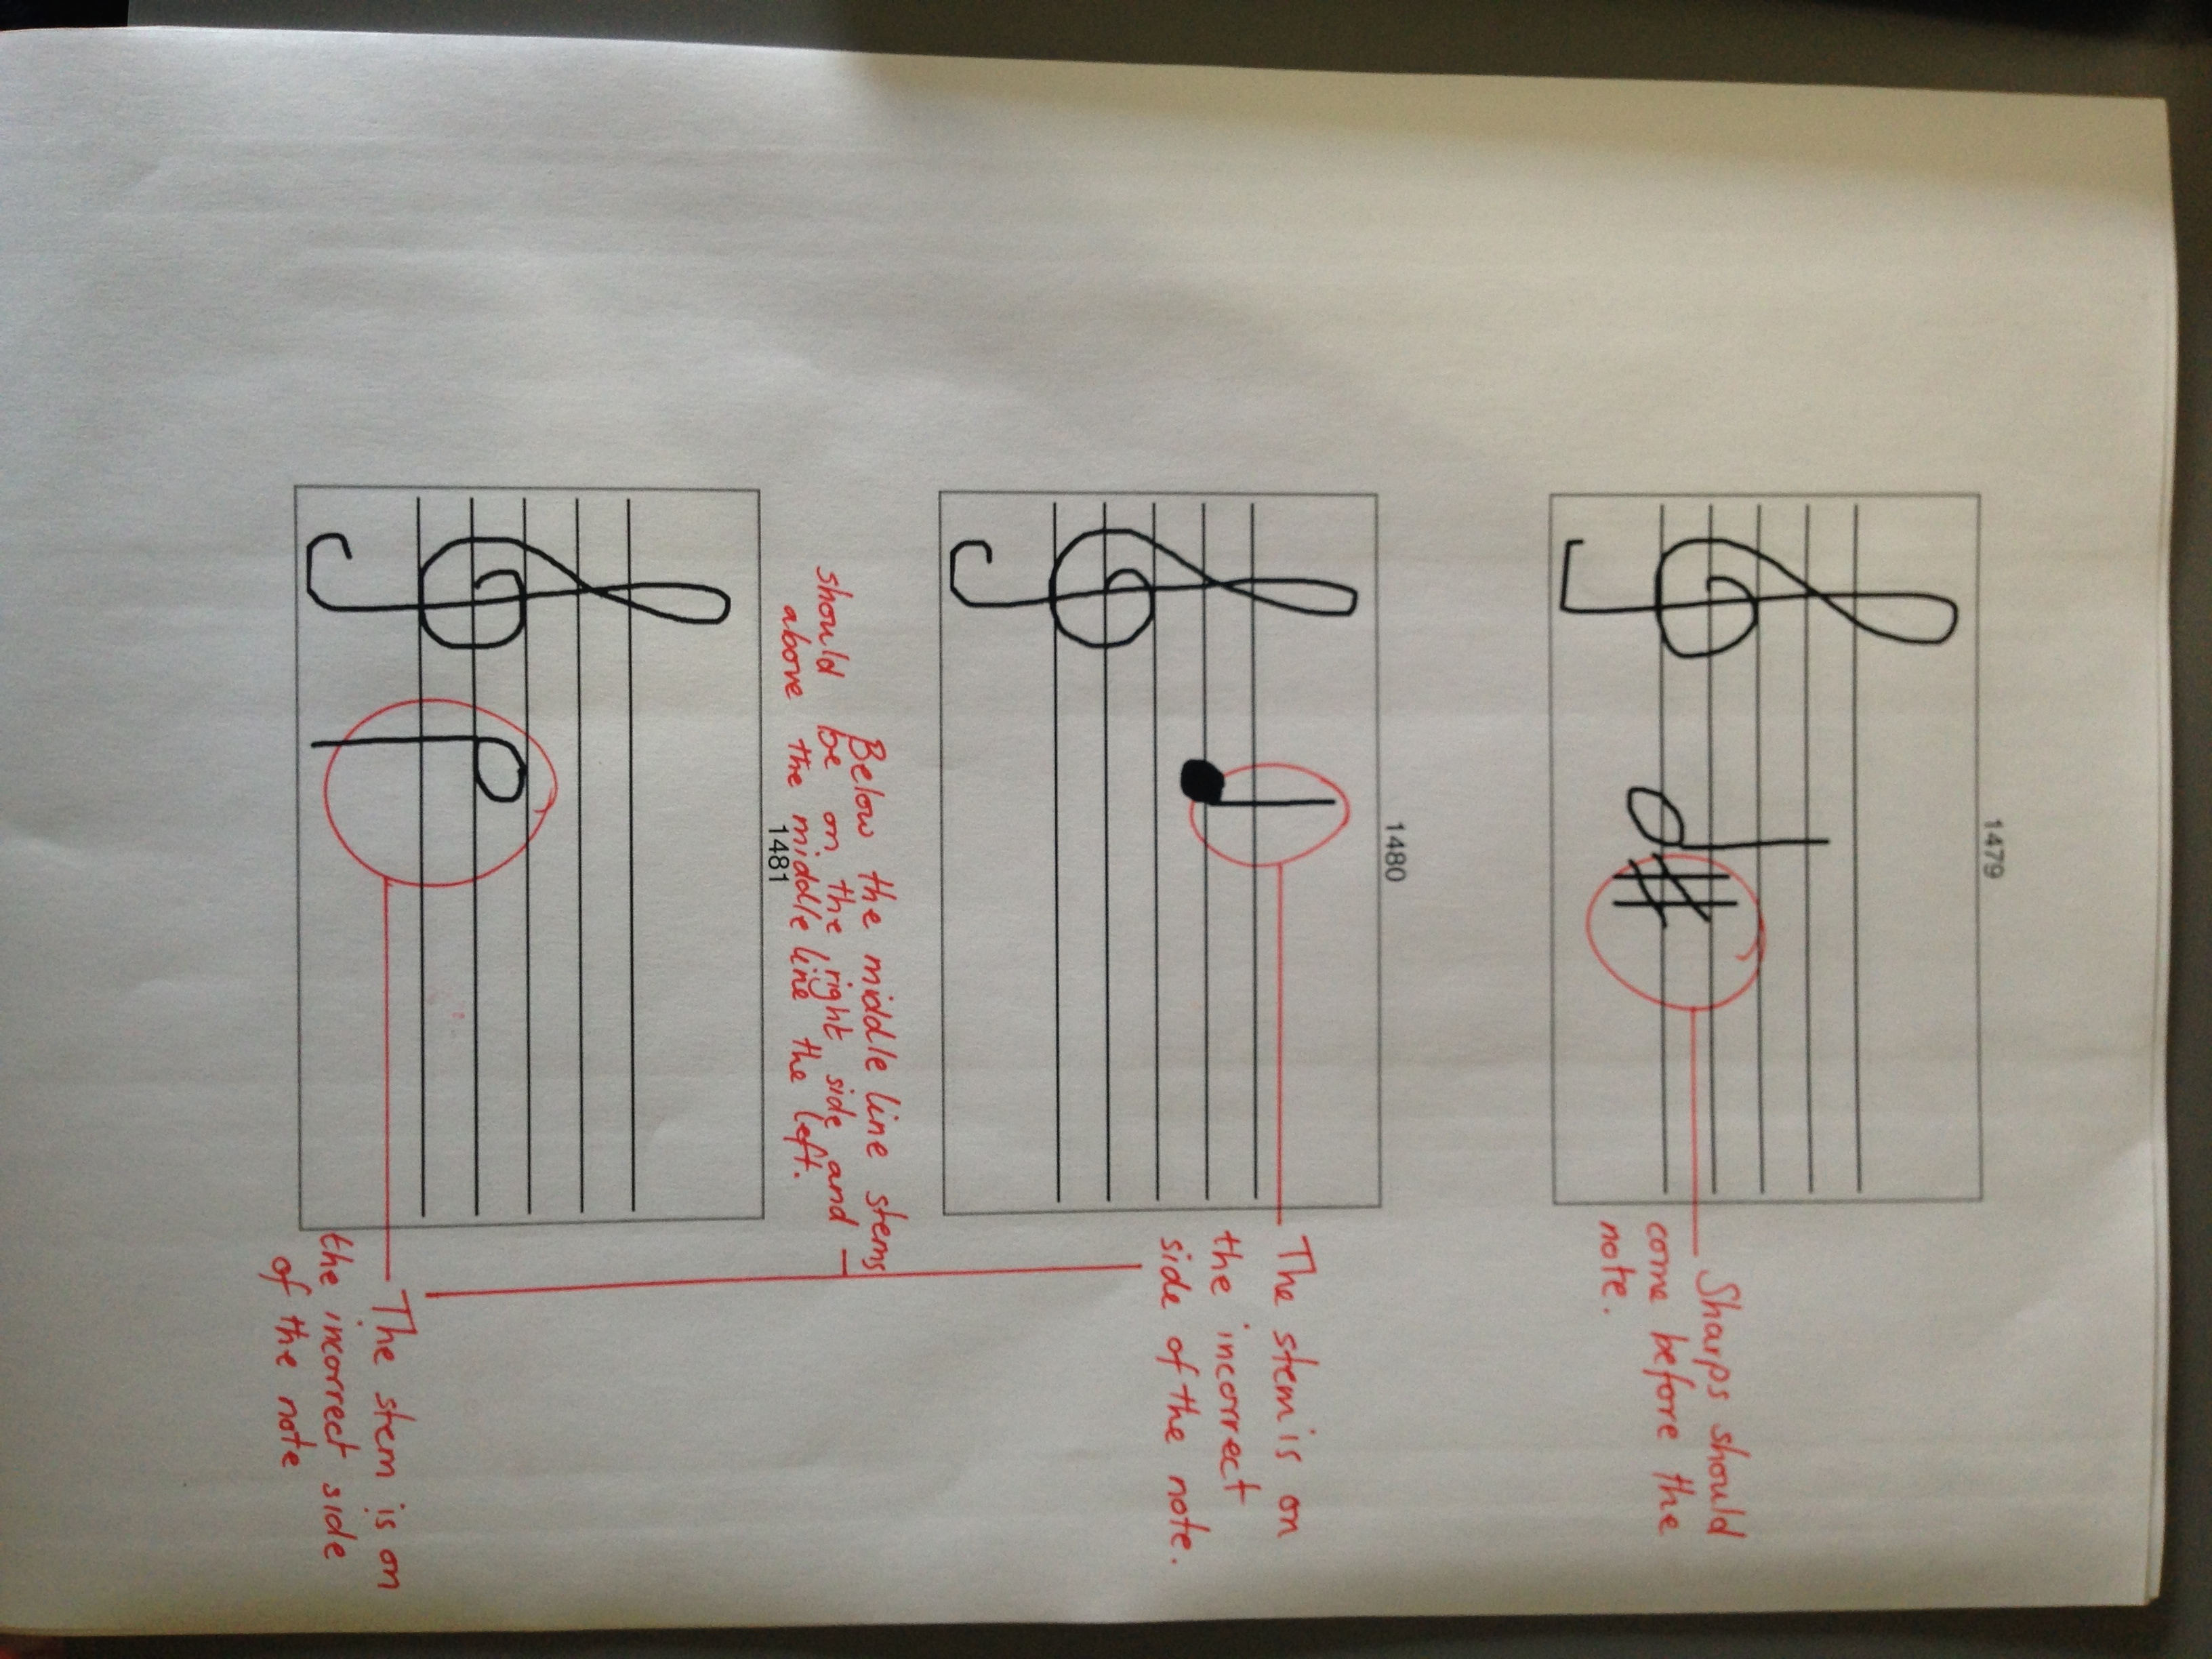
\includegraphics[width=.45\linewidth]{gfx/photos/teacher-sheet-1.jpg}}
  \rot{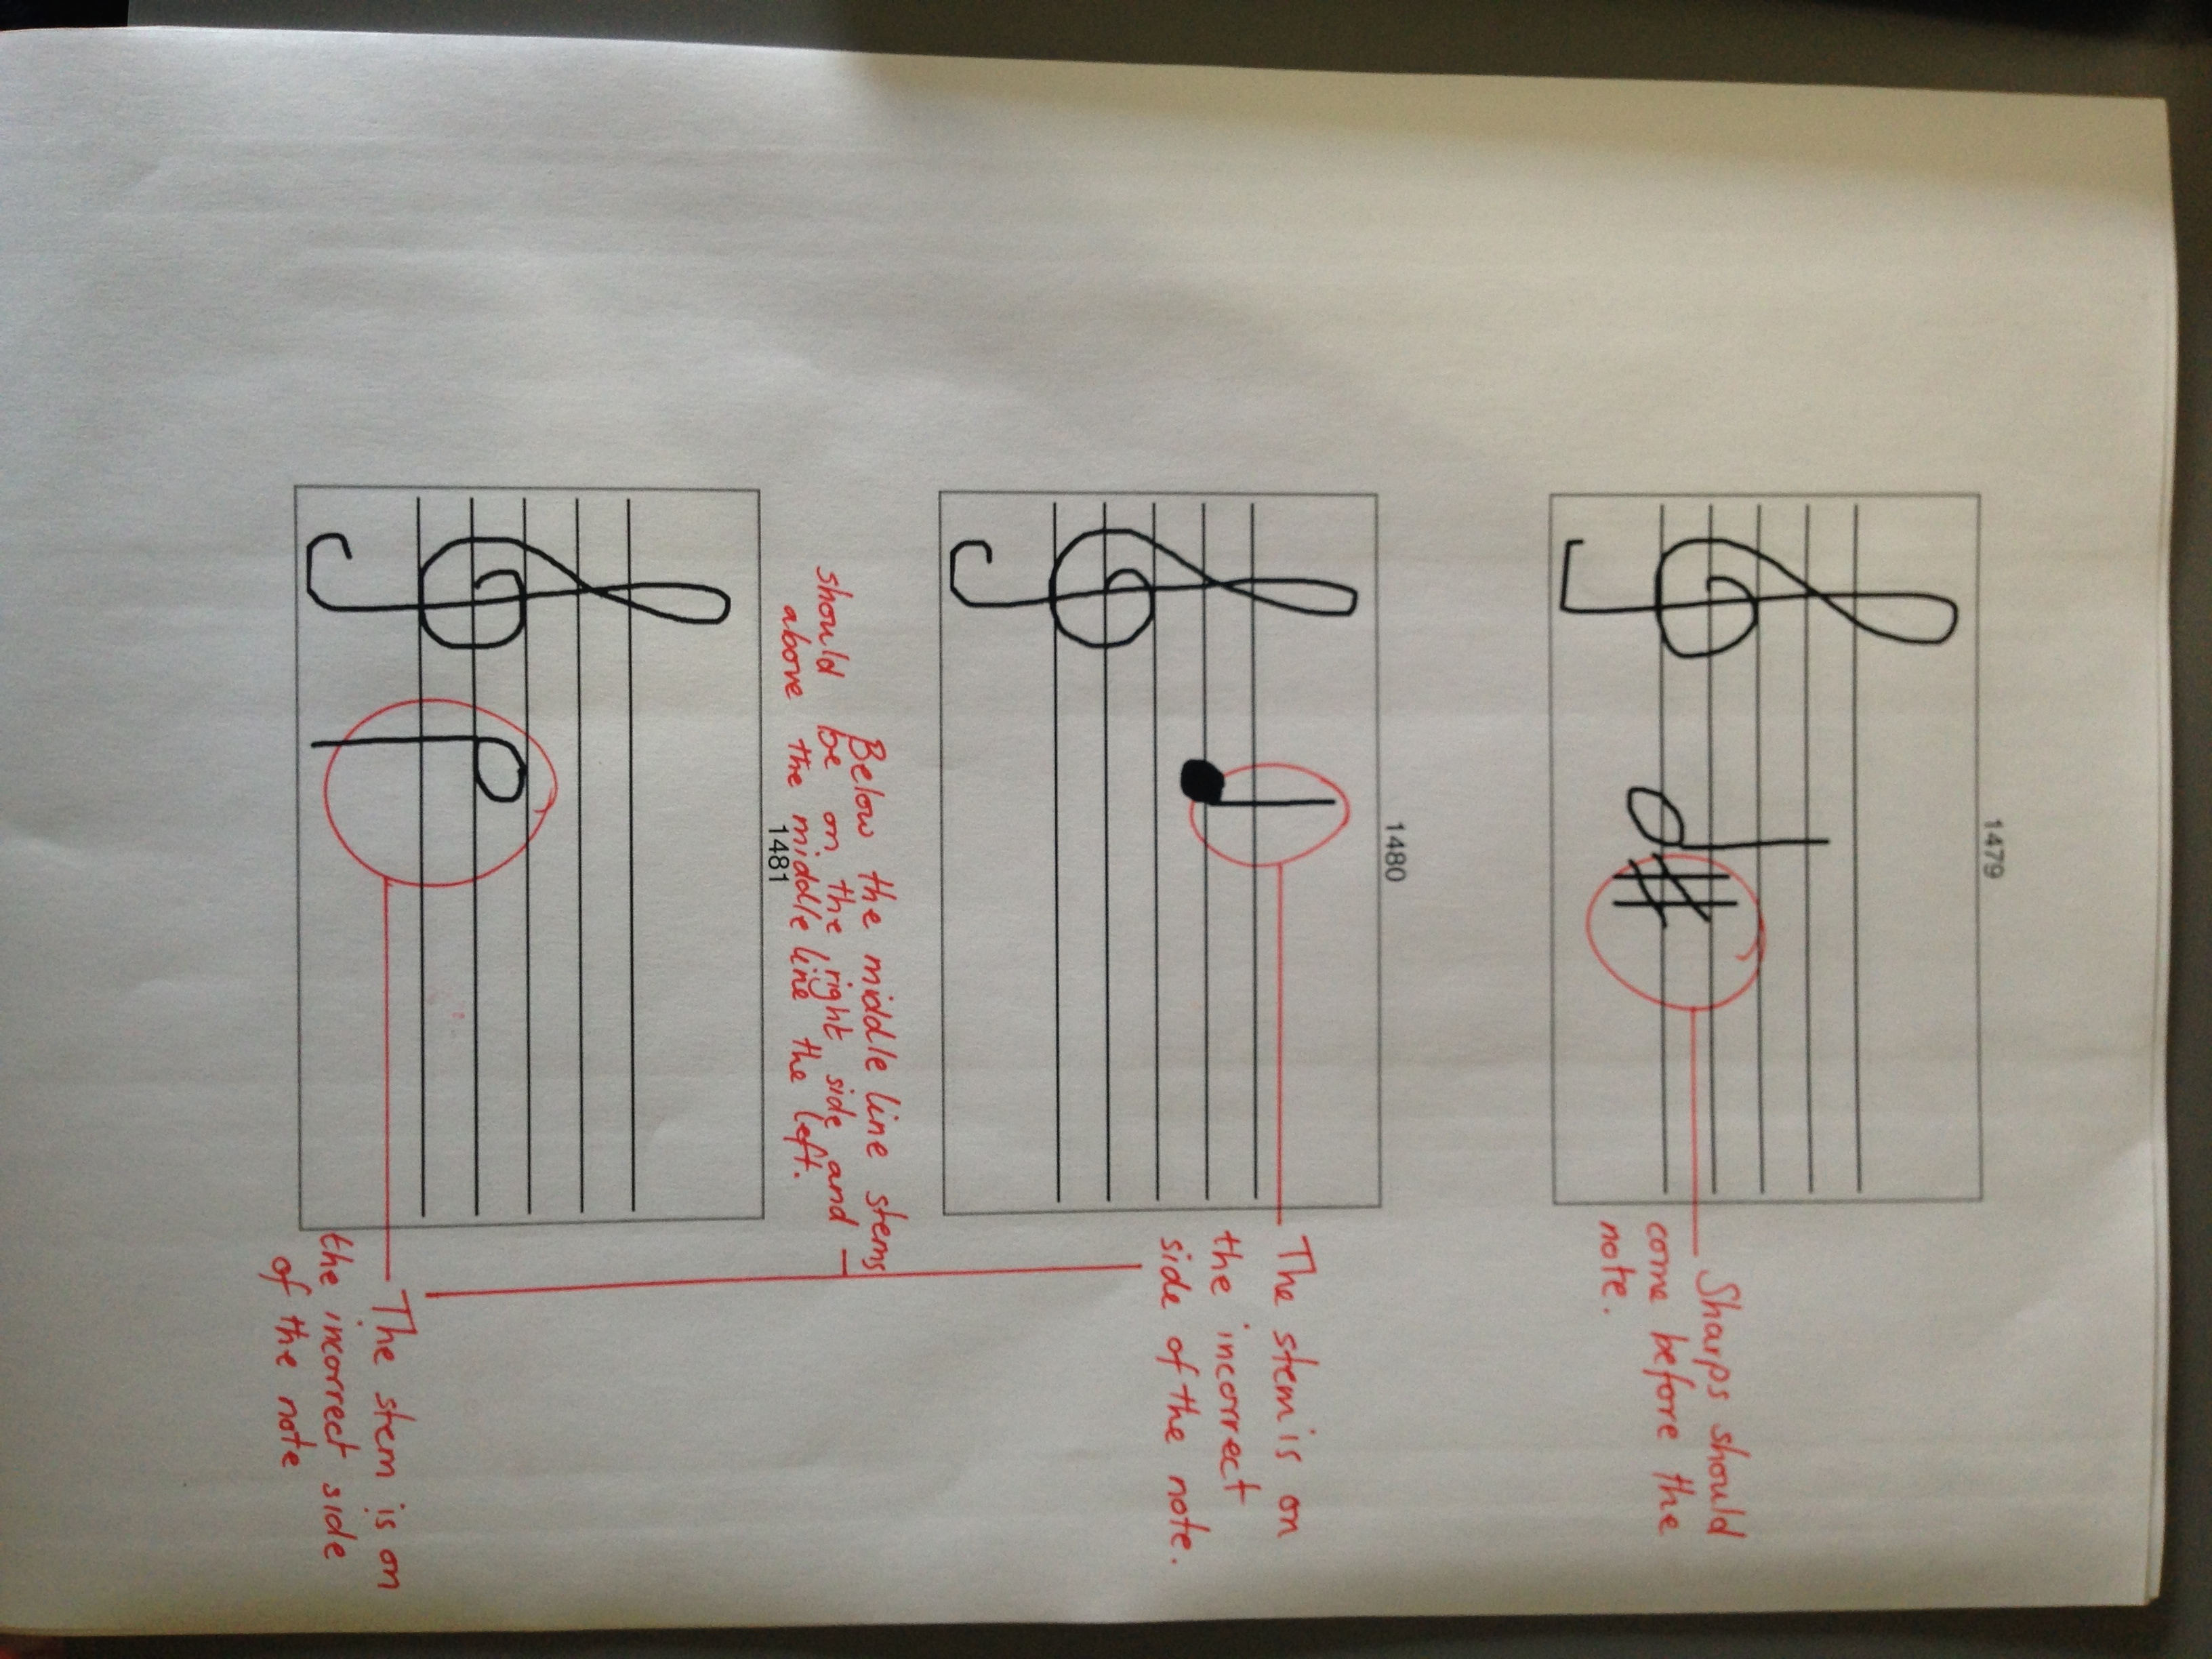
\includegraphics[width=.45\linewidth]{gfx/photos/teacher-sheet-2.jpg}}
  \caption{Examples of teacher-annotated manuscript}
  \label{fig:teacher-sheet}
\end{figure}

Quaver tails are given as an example till I move everything else down.

\subsection{Quavers}

\subsubsection{Quaver Tail Side}

\begin{figure}[H]
  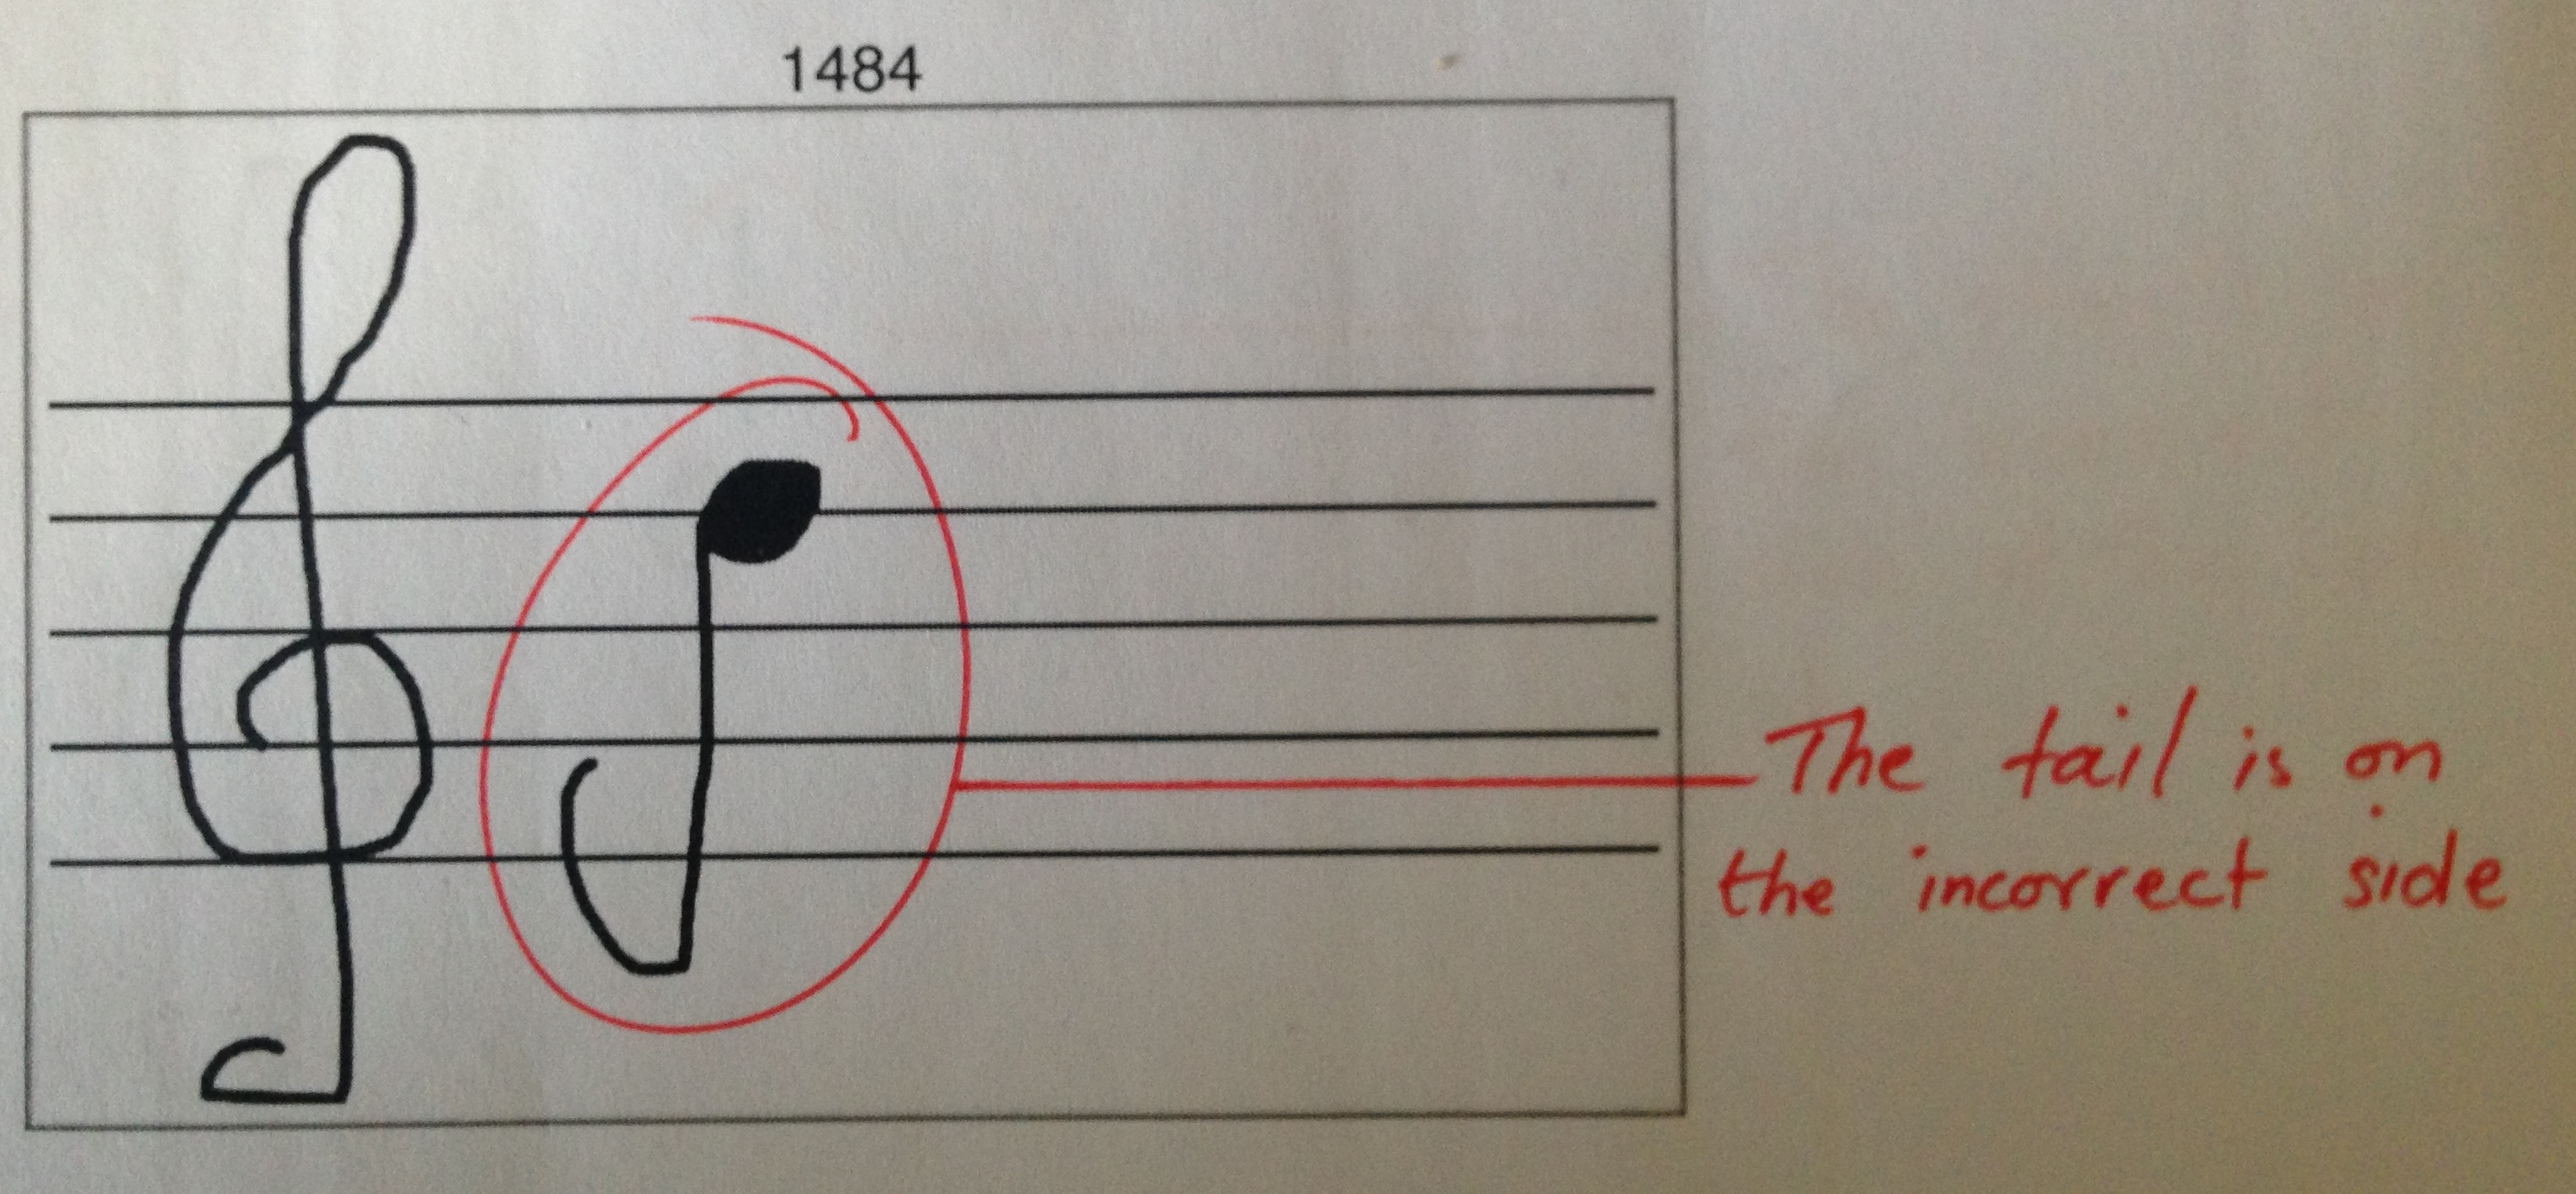
\includegraphics[width=\linewidth]{gfx/photos/teacher-bad-quavertail-side.jpg}
  \caption{Teacher's annotation of a bad quaver tail side}
  \label{fig:teacher-example-quaver-wrong-side}
\end{figure}
